\documentclass[12pt,a4paper]{scrartcl} 
\usepackage[utf8]{inputenc}
\usepackage[english,russian]{babel}
\usepackage{indentfirst}
\usepackage{misccorr}
\usepackage{graphicx}
\usepackage{indentfirst}
\usepackage{amsmath}
\begin{document}
 \begin{titlepage}
  \begin{center}
   \large
   МИНИСТЕРСТВО НАУКИ И ВЫСШЕГО ОБРАЗОВАНИЯ РОССИЙСКОЙ ФЕДЕРАЦИИ
   
   Федеральное государственное бюджетное образовательное учреждение высшего образования
   
   \textbf{АДЫГЕЙСКИЙ ГОСУДАРСТВЕННЫЙ УНИВЕРСИТЕТ}
   \vspace{0.25cm}
   
   Инженерно-физический факультет
   
   Кафедра автоматизированных систем обработки информации и управления
   \vfill

   \vfill
   
   \textsc{Отчет по практике}\\[5mm]
   
   {\LARGE Разбиение видео на кадры с применением FFmpeg. \textit{Вариант 8}}
   \bigskip
   
   2 курс, группа 2ИВТ1-1
  \end{center}
  \vfill
  
  \newlength{\ML}
  \settowidth{\ML}{«\underline{\hspace{0.7cm}}» \underline{\hspace{2cm}}}
  \hfill\begin{minipage}{0.5\textwidth}
   Выполнил:\\
   \underline{\hspace{\ML}} Д.\,Д.~Давтян\\
   «\underline{\hspace{0.7cm}}» \underline{\hspace{2cm}} 2024 г.
  \end{minipage}%
  \bigskip
  
  \hfill\begin{minipage}{0.5\textwidth}
   Руководитель:\\
   \underline{\hspace{\ML}} С.\,В.~Теплоухов\\
   «\underline{\hspace{0.7cm}}» \underline{\hspace{2cm}} 2024 г.
  \end{minipage}%
  \vfill
  
  \begin{center}
   Майкоп, 2024 г.
  \end{center}
 \end{titlepage}
 
% Содержание
\section{Введение}
\label{sec:intro}


\subsection{Формулировка цели}
Целью данной работы является написание программы для разбиения видео на кадры с применением FFmpeg.

\subsubsection{Теория}
FFmpeg — это мощный инструмент для обработки аудио и видео, предоставляющий возможности записи, конвертации и трансляции мультимедийных файлов. Основной утилитой FFmpeg является командная строка ffmpeg, которая позволяет выполнять разнообразные операции с мультимедийными файлами.\\
\\
Основные функции FFmpeg:
\begin{itemize}
    \item Преобразование форматов: Конвертация файлов из одного формата в другой.
    \item Преобразование форматов: Конвертация файлов из одного формата в другой.
    \item Разбиение видео на кадры: Извлечение каждого кадра из видеофайла и сохранение его как отдельное изображение.
    \item Слияние файлов: Объединение нескольких аудио или видео файлов в один.
\end{itemize} 
Основные комманды FFmpeg:

\begin{itemize}
    \item Конвертация видео из одного формата в другой: \\
        Пример: ffmpeg -i input.mp4 output.avi
    \item Извлечение аудио дорожки из видеофайла:\\
        Пример: ffmpeg -i input.mp4 -q:a 0 -map a output.mp3
    \item Объединение аудио и видео файлов в один:\\
        Пример: ffmpeg -i video.mp4 -i audio.mp3 -c:v copy -c:a aac output.mp4
    \item  Изменение разрешения видео:\\
        Пример: ffmpeg -i input.mp4 -vf scale=1280:720 output.mp4
    \item  Изменение битрейта видео:\\
        Пример: ffmpeg -i input.mp4 -b:v 1M output.mp4
    \item  Извлечение каждого кадра из видео и сохранение их как изображения:\\
        Пример: ffmpeg -i input.mp4 output\textunderscore frame\textunderscore \%04d.png
    \item Обрезка видео по времени:\\
        Пример: ffmpeg -i input.mp4 -ss 00:00:10 -t 00:00:20 -c copy output.mp4
    \item Добавление водяного знака к видео:\\
        Пример: ffmpeg -i input.mp4 -i watermark.png -filter\textunderscore complex "overlay=10:10" output.mp4
    \item Изменение частоты кадров видео:\\
        Пример: ffmpeg -i input.mp4 -r 30 output.mp4
    \item Нормализация аудио уровня:\\
        Пример: ffmpeg -i input.mp4 -filter:a "volume=1.5" output.mp4
     
\end{itemize}

\section{Ход работы}
\subsection{Код выполненной программы}
\sloppy
\begin{verbatim}

#include <iostream>
#include <string>
#include <cstdlib>

int main() {
    setlocale(LC_ALL, "ru");
    std::string videoPath;
    std::string outputDir;

    std::cout << "Введите путь к видеофайлу: ";
    std::getline(std::cin, videoPath);

    std::cout << "Введите папку для сохранения кадров: ";
    std::getline(std::cin, outputDir);

    std::string command = "ffmpeg -i \"" + videoPath + "\" \"" + outputDir +
        + "/frame_%04d.png\"";

    int result = std::system(command.c_str());

    if (result == 0) {
        std::cout << "Кадры успешно сохранены в папку: " << outputDir << std::endl;
    }
    else {
        std::cerr << "Ошибка при выполнении команды FFmpeg." << std::endl;
    }

    return 0;
}


\end{verbatim}

\begin{figure}[h]
 \centering
 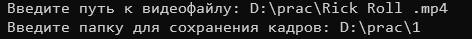
\includegraphics[width=0.8\textwidth]{dan.png}
 \caption{Ввод данных}\label{fig:par}
\end{figure}

\begin{figure}[h]
 \centering
 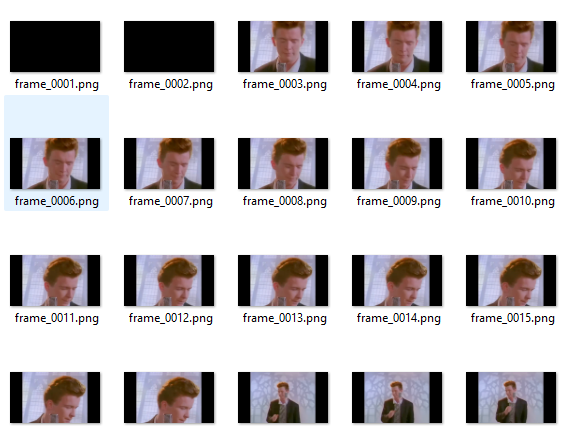
\includegraphics[width=0.8\textwidth]{result.png}
 \caption{Результат работы}\label{fig:par}
\end{figure}

\end{document}